\section{Robustness of a standard NN}
In this work the MLM analyzed is a BNN. However, before diving into robustness evaluation of BNNs we will introduce an approach to assess the robustness a standard NN classifier, based on the work of Arcaini et al. \cite{9176802}.

Building upon the concepts introduced in the previous section, for a NN classifier the correctness can be defined as the accuracy, i.e. the ration between the number of correct predictions and the total samples number given to the network. More formally, given a classifier C and a set of input D, the accuracy of C on P is defined as:

\[
	acc(C,D) = \frac{|{d \in D | C(d) = correctLabel(d)}|}{|D|}
\] 

where $C(d)$ represents the classification output for the input $p$, and $correctLabel(d)$ gives the correct label for the input $d$.

The common approach for evaluating NNs robustness is to asses the network accuracy when altered data are given as input.
In existing literature, the robustness of NNs is typically determined and measured through the utilization of \textit{adversarial} examples \cite{rnnvta2018} \cite{9785704}. These are inputs specifically designed to be challenging for the network under test, exploiting its internal structure \cite{759851e20d2e47aaad2a560211f6a126}, resulting in what is known as adversarial robustness.
While assessing adversarial robustness is important for ensuring the system security against external attacks, it is not sufficient to define a network entirely robust.
In the real world, the occurrence of adversarial examples is improbable \cite{8805674}.
Adversarial robustness is an important quality for the protection of the system from external attacks, in fact it is usually related to the security. However, the possible alterations can be due to dynamic environmental factors beyond intentional attacks. These alterations are the most common to happen. Consequently, assessing the network robustness against real world perturbations holds significant importance.

Based on these considerations, it is possible to give a general definition of alteration.

\begin{definition} (Alteration).
	An \textit{alteration} of type \textit{A} of an input \textit{t} is a transformation of \textit{t} that mimics the possible effect on \textit{t} when a problem occurs in reality. The range of plausible alterations of type A is identified as $[L_A, U_A]$; Given a dataset $D$, $D^{A_i}$ denotes the set obtained by altering all the data in $D$ with an alteration of type A with \textit{level} $i \in [L_A, U_A]$.
	The range of plausible alterations must be defined in a manner that guarantees the existence of a level $u$ for which $D^{A_u} = D$, signifying the absence of alteration. 
\end{definition}
 
The notion of "level" refers to the intensity of the applied transformation. For instance, consider the addition of white noise to the input. In this context, the variance of the added noise serves as a parameter that determines the level of intensity for the transformation.

This concept underlines the complexity in defining robustness. As highlighted by the introduction of the alteration concept, a network robustness is not a straightforward quantity to define. Rather, it refers to the specific alteration type under consideration. Furthermore, within each alteration type, there can exist multiple levels of intensity. Consequently, a network can be robust in relation to a particular alteration type and corresponding intensity level.

Following these considerations we introduce the robustness definition proposed in \cite{9176802}, which takes into account all these aspects. 

\begin{definition}\label{def:rob} (Robustness)
	The robustness $rob_A(C,D) \in [0,1]$ of a classifier $C$ w.r.t. alteration of type A in the range $[L_A, U_A]$ on a dataset $D$ is defined the percentage of alteration values for which the accuracy is above a threshold $\Theta$. Formally:
	\[
		rob_A(C,D) = \frac{\int_{L_A}^{U_A} H(acc(C,D^{A_i}) - \Theta) \ di}{L_A - U_A}
	\]
	
	Where $\Theta$ is the minimum accuracy accepted and $ H(x) = \begin{cases}
		1 \ for \ x \geq 0\\
		0 \ for \ x < 0\\
	\end{cases}$.
\end{definition}

The parameter $\Theta$ can be chosen in various ways, e.g. from the specific application requirements. \Fig~\ref{fig:rob_example} presents a graphical example showcasing the application of the introduced definition using a $\Theta = 85\%$.

\begin{figure}[h]
	\centering
	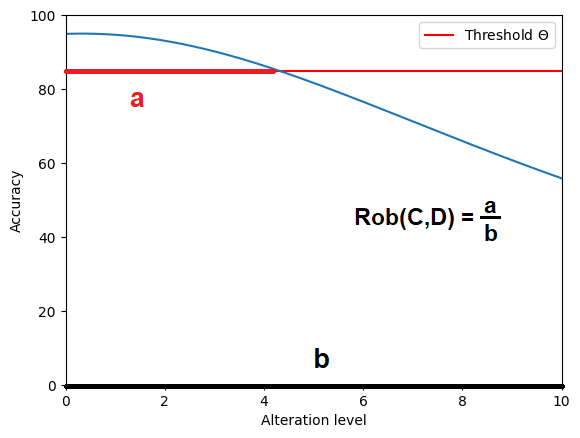
\includegraphics[width=0.7\linewidth]{ImageFiles/ANNRob/rob_example}
	\caption{Example of a robustness evalutation using the approach in \cite{9176802} with $\Theta=85\%$}
	\label{fig:rob_example}
\end{figure}

However, implementing this definition would necessitate having prior knowledge of the analytical expression of the \textit{acc} function. Given that computing accuracy across an infinite number of alteration levels is infeasible, the evaluation is confined to a finite set of alteration levels. This results in an approximate measurement of robustness. This approximation is better as the number of levels considered increases. An example of this approach is illustrated in \Fig~\ref{fig:rob_example_discr}.

\begin{figure}[h]
	\centering
	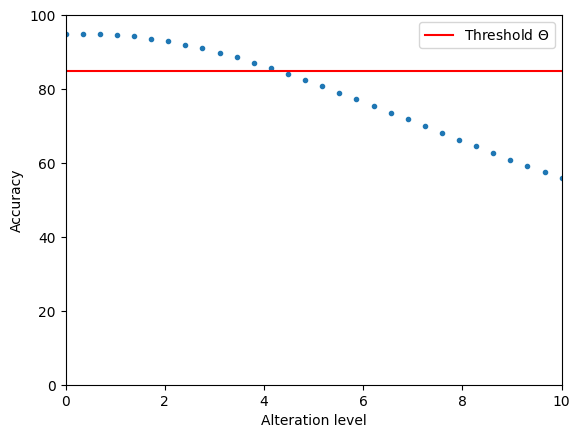
\includegraphics[width=0.7\linewidth]{ImageFiles/ANNRob/rob_example_discr}
	\caption{Example of approximate robustness evalutation using the approach in \cite{9176802} with $\Theta=85\%$}
	\label{fig:rob_example_discr}
\end{figure}

Although the provided formula could serves as a measure of robustness, it has certain limitations. Specifically, it penalizes any degradation in accuracy in the same way. For instance, whether the observed accuracy decreases by 1\% or 10\% relative to the nominal accuracy, the formula treats both scenarios identically. Furthermore, it assigns equal importance to all alteration levels. However, it could be that some alteration levels might occur more frequently than others. In such cases, it is more realistic to consider the probability of each alteration level to occur. In order to overcome these limitations an extension to the proposed definition in \cite{9176802} will be introduced.

The idea to extend the formula is to replace the $H$ function with a generic function denoted as $tol$. This introduces the concept of \textit{tolerance}, proposed in \cite{9787878}. 

\begin{definition} (Tolerance)
	Within the context of classification, the tolerance is a function such that:
	
	\[
	\begin{cases}
		0 \le tol(x) \le 1 , \ for \ x > 0\\
		tol(x) = 0, \ for \ x < 0
	\end{cases}	
	\]
\end{definition}

The tolerance function can be interpreted as the reward given for being above the threshold $\Theta$. It can be defined in several ways, based also on the specific application and the desired performance. Here there will be presented some classical functions the could be applied:

\begin{itemize}
	\item \textit{Uniform tolerance}: With this function all the accuracy values above $\Theta$ are rewarded equally. This is the case leads back to formula in \Def~\ref{def:rob}. Formally: 
	\[
		tol(acc(C,D^{A_i}) - \Theta) = H(acc(C,D^{A_i}) - \Theta)
	\]
	Where $H$ is the Heaviside Step function. This is suitable for the cases when it is important just to stay above the threshold, no matter how much.
	\item \textit{Linear tolerance}: This function gives a reward proportional to the distance $\Theta$, higher accuracy values are more tolerated the lower ones. Formally: 
	\[
		tol(acc(C,D^{A_i}) - \Theta) = \frac{max(min(acc(C,D^{A_i}), maxAcc) - \Theta, 0)}{maxAcc - \Theta}
	\]
	This function is adapt to cases when it is not only necessary to be above the threshold but to have some margin above it as well. The denominator is added for normalization, \textit{maxAcc} refers to the accuracy with maximum tolerance, in general it can be $100\%$, but lower values may make sense as well, such as the nominal accuracy. There could be some cases when $maxAcc$ is lower than some accuracy values. This leads to a situation where we want to reward all the values above $maxAcc$ in the same way. This is useful in applications where it is important to stay above $\Theta$ for as much as possible alteration levels rather than having very high accuracy that drops down steeply. $maxAcc$ is an important parameter to define since it sets the baseline respect which to evaluate the robustness. Alternatively, one might opt for the network accuracy under \textit{nominal} conditions, i.e. without any alteration. This choice would lead to a metric that quantifies the performance degradation when the network operates within an perturbed environment. 
\end{itemize}

With this notions in mind it is now possible to introduce e first robustness definition extension.

\begin{definition} (Robustness extension 1).
	Let $C$ be a classifier and $tol(x)$ a tolerance function.
	The robustness $rob_A(C,D) \in [0,1]$ of a classifier $C$ w.r.t. alteration of type A in the range $[L_A, U_A]$ on a dataset $D$ is defined formally as:
	\[
		rob_A(C,D) = \frac{\int_{L_A}^{U_A} tol(acc(C,D^{A_i}) - \Theta) \ di}{(U_A - L_A)}
	\]
\end{definition}

This is a more general definition which tackles some previous limitations such as the importance given to the accuracy values. With a generic function it is possible to evaluate the robustness w.r.t. the preferred criteria.

In \Fig~\ref{fig:rob1_tol} are reported two examples of robustness evaluation. \Fig~\ref{fig:rob1_uni_tol} shows the use of a uniform tolerance, which conducts to the original definition. \Fig~\ref{fig:rob1_lin_tol} shows the use of a linear tolerance instead, using as maximum accuracy $100\%$, in other words this evaluation computes the robustness as the area between the accuracy and the threshold divided by the ideal area, which is the one between the maximum accuracy and the threshold.

\begin{figure}[h]
	\centering
	\begin{subfigure}{.5\textwidth}
		\centering
		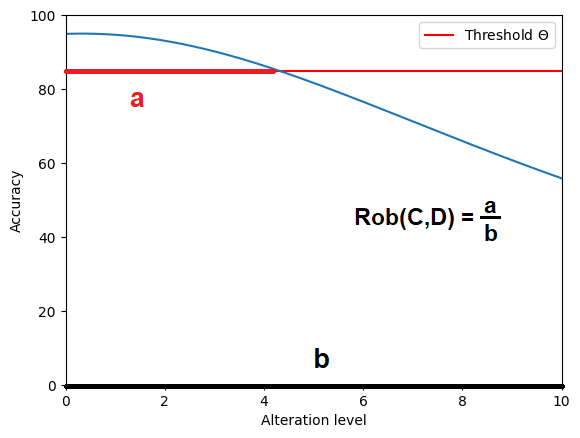
\includegraphics[width=0.9\linewidth]{ImageFiles/ANNRob/rob_example}
		\caption{Application of a uniform tolerance for robustness evaluation}
		\label{fig:rob1_uni_tol}
	\end{subfigure}%
	\begin{subfigure}{.5\textwidth}
		\centering
		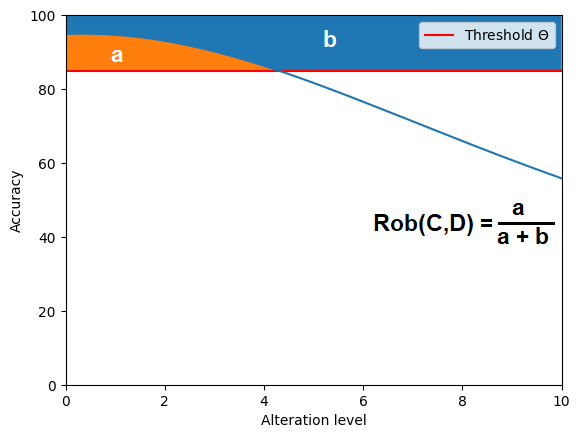
\includegraphics[width=0.9\linewidth]{ImageFiles/ANNRob/rob1_lin_tol}
		\caption{Application of a linear tolerance for robustness evaluation}
		\label{fig:rob1_lin_tol}
	\end{subfigure}
	\caption{Example of robustness evaluation with the extended formula using $\Theta=85\%$}
	\label{fig:rob1_tol}
\end{figure}

Although this definition is more general, it treats all accuracy values beyond the threshold uniformly. In essence, regardless of the degradation extent, once the threshold is crossed, all accuracy values contribute equally to the robustness metric. This can be better visualized in \Fig~\ref{fig:rob_problem_1}. In this scenario, the application of the proposed formula would yield approximately the same robustness value for both cases. However, it is evident that the blue accuracy represents a less robust network than the orange one. Furthermore, in certain applications, a strict threshold might not be applicable, or it could be necessary to ensure that even when accuracy falls below the threshold, it doesn't deviate too far from the nominal accuracy.

\begin{figure}[h]
	\centering
	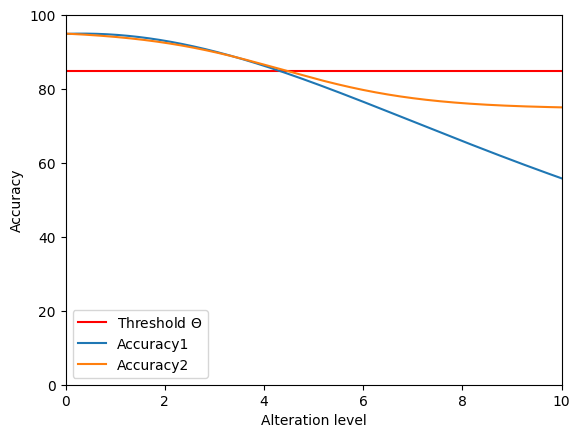
\includegraphics[width=0.8\linewidth]{ImageFiles/ANNRob/rob_problem_1}
	\caption{Example of two accuracy functions with a similar behavior only before the threshold}
	\label{fig:rob_problem_1}
\end{figure}

To overcome this limitation, the concept of "penalization" will be introduced. The idea is to incorporate an additional term into the integral that penalizes deviations below the threshold.

\begin{definition} (Penalization).
	Within the context of classification, the penalization is a function, denoted as $dep(x)$, such that:
	\[
		\begin{cases}
			0 \le dep(x) \le 1 , \ for \ x \le 0\\
			dep(x) = 0, \ for \ x > 0
		\end{cases}	
	\]
\end{definition}

This function quantifies the amount of penalization for crossing the threshold $\Theta$. Similarly to the tolerance concept, custom functions can be defined based on specific requirements. Here are some examples:
\begin{itemize}
	\item Zero penalization: This function represents trivially the absence of penalization, essentially reverting to the initial robustness extension definition:
	\[
		dep(acc(C,D^{A_i}) - \Theta) = 0
	\]
	
	\item Linear penalization: This function behaves similarly to the tolerance case, penalizing proportionally to the distance from the threshold:
	\[
		dep(acc(C,D^{A_i}) - \Theta) = \frac{max(-(acc(C,D^{A_i}) - \Theta), 0)}{\Theta}
	\]
	\item Logarithmic penalization: The intuition behind this function is to start penalizing as soon as the threshold is crossed but not drastically increase penalization for very low accuracy values, since generally those cases represent similarly bad situations at a comparable severity level. Formally:
	\[
		dep(acc(C,D^{A_i}) - \Theta) = \frac{max(log_{10}(-(acc(C,D^{A_i}) - \Theta) + 1),0)}{log_{10}(\Theta + 1)}
	\]
	The division by $log_{10}(\Theta + 1)$ normalizes the function so that the worst case, where accuracy is $0\%$, results in a penalization of $1$.
	\Fig~\ref{fig:log_penalization} shows an example of this function using an $85\%$ threshold. It is apparent that the worst case occurs when x = $-85\%$, i.e. zero accuracy, and the penalization is $1$, the maximum.
\end{itemize}

\begin{figure}[h]
	\centering
	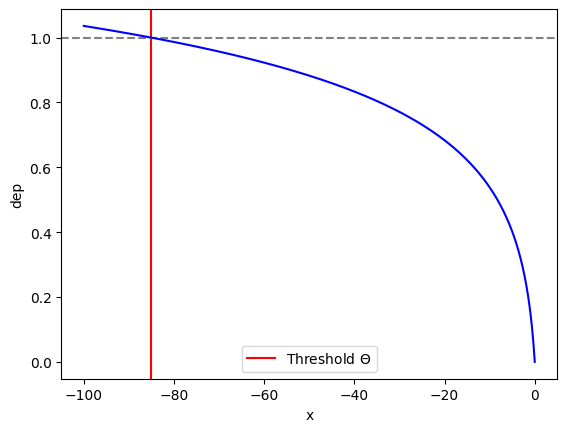
\includegraphics[width=0.7\linewidth]{ImageFiles/ANNRob/log_penalization}
	\caption{Logarithmic penalization function assuming $\Theta=85\%$}
	\label{fig:log_penalization}
\end{figure}

With this concept in mind it possible to introduce a second extension of the robustness definition that incorporates this aspect as well.

\begin{definition}\label{def:rob2} (Robustness extension 2).
	Let $C$ be a classifier, $tol(x)$ a tolerance function and $dep(x)$ a penalization function.
	The robustness $rob_A(C,D) \in [0,1]$ of a classifier $C$ w.r.t. alteration of type A in the range $[L_A, U_A]$ on a dataset $D$ is defined formally as:
	\[
		rob_A(C,D) = \frac{\int_{L_A}^{U_A} tol(acc(C,D^{A_i}) - \Theta) - dep(acc(C,D^{A_i}) - \Theta)\ di}{2 \cdot (U_A - L_A)} + \frac{1}{2}
	\]
	where $\Theta$ is a threshold referring to minimum accuracy accepted.
\end{definition}

In this new definition, the addition of $\frac{1}{2}$ serves to prevent negative values.

To provide some intuition, consider the worst-case scenario where accuracy consistently falls below the threshold, assuming maximum penalization.
The term 
\[
	\frac{\int_{L_A}^{U_A} tol(acc(C,D^{A_i}) - \Theta) - dep(acc(C,D^{A_i}) - \Theta)\ di}{(U_A - L_A)}
\] 

would give $-1$. With the additional terms, this result is adjusted to $-\frac{1}{2} + \frac{1}{2} = 0$, which aligns with the intended measure.
It's worth noting that only adding $1$ would not sufficient, as in the best-case scenario, $\frac{\int_{L_A}^{U_A} tol(acc(C,D^{A_i}) - \Theta) - dep(acc(C,D^{A_i}) - \Theta)\ di}{(U_A - L_A)}$ would yield $1$.
Without the division by $2$, this would lead to $1 + 1 = 2$, which falls outside the desired range of $[0, 1]$.

The last definition is slightly more complex but it can capture different aspects by choosing only two functions: tolerance and penalization. An example of the application os this formula is shown in \Fig~\ref{fig:rob_lin_tol_lin_pen}. In this example both the tolerance and penalization are linear. It is possible to see immediately the difference with the previous case, depicted in \Fig~\ref{fig:rob1_uni_tol}, which is the green area, subtracted in the numerator. 

The latest definition is slightly more intricate, but it offers the flexibility to include various aspects by choosing just two functions: tolerance and penalization. An example of its application is illustrated in \Fig~\ref{fig:rob_lin_tol_lin_pen}. In this instance, both the tolerance and penalization functions are linear. It is possible to immediately note the difference with the previous case, depicted in \Fig~\ref{fig:rob1_uni_tol}, which is the green area, subtracted in the numerator. 

\begin{figure}[h]
	\centering
	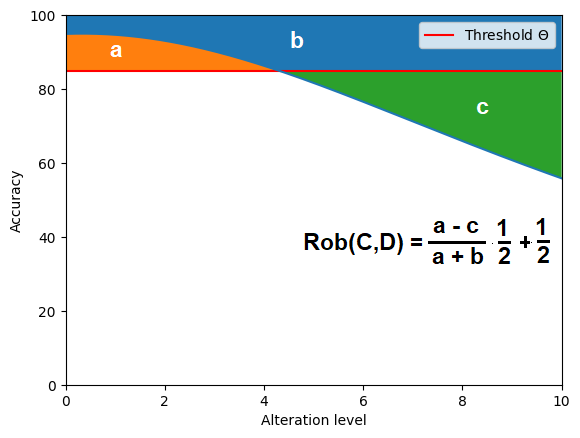
\includegraphics[width=0.7\linewidth]{ImageFiles/ANNRob/rob_lin_tol_lin_pen}
	\caption{Example of the application of robustness extension definition 2 with $\Theta=85\%$}
	\label{fig:rob_lin_tol_lin_pen}
\end{figure}

Until now, the primary emphasis has been on accuracy, more precisely about how to reward or penalize the accuracy values concerning a minimum acceptable value $\Theta$ and a desired value $maxAcc$. These discussions were operated under the hidden assumption that all alteration levels have an equal likelihood of occurring. However, in reality, certain alteration levels may be more probable than others. Consequently, it becomes logical to incorporate the probability distribution of these different levels when calculating the robustness.

\begin{definition}(Alteration probability).
	Given an alteration of type $A$, $p_A$ identifies the the probability distribution of the alteration level having
	as support the interval $[L_A, U_A]$. 
\end{definition}

Usually finding the actual probability distribution is challenging. In these cases it is possible to define a distribution that reflects the significance attributed to each alteration level. Several typical functions that can be used for this purpose include:

\begin{itemize}
	\item Uniform: This distribution assigns equal importance to all alteration levels, as exemplified in \Fig~\ref{fig:unifo_prob}. The mathematical expression for this distribution is:
	\[
		p_A(i) = \begin{cases}
			\frac{1}{U_A - L_A}, \ for \ L_A \le i \le U_A\\
			0, \ \ \ \ otherwise
		\end{cases}
	\]
	\item Linear: As depicted in \Fig~\ref{fig:lin_prob}, this function assigns a higher probability to lower alteration levels through a linear approximation:
	\[
		p_A(i) = \begin{cases}
			\frac{2}{(U_A - L_A)^2}\cdot (U_A - i), \ for \ L_A \le i \le U_A\\
			0, \ \ \ \ otherwise
		\end{cases}
	\] 
	\item Exponential: This distribution also assigns higher probability to lower alteration levels but it employs an exponential function to assign lower probabilities to higher levels, as seen in \Fig~\ref{fig:exp_prob}. The mathematical expression is:
	\[
		p_A(i) = \begin{cases}
			-\frac{1}{a^{-L_A} - a^{-U_A}}\cdot a^{-i}, \ for \ L_A \le i \le U_A\\
			0, \ \ \ \ otherwise
		\end{cases}
	\]
	where $a$ defines the slope of the distribution. An example is shown in \Fig~\ref{fig:exp_prob}.
\end{itemize}

These distributions can help reflect the importance given to each alteration level based on the specific application or context.

\begin{figure}[h]
	\centering
	\begin{subfigure}{.33\textwidth}
		\centering
		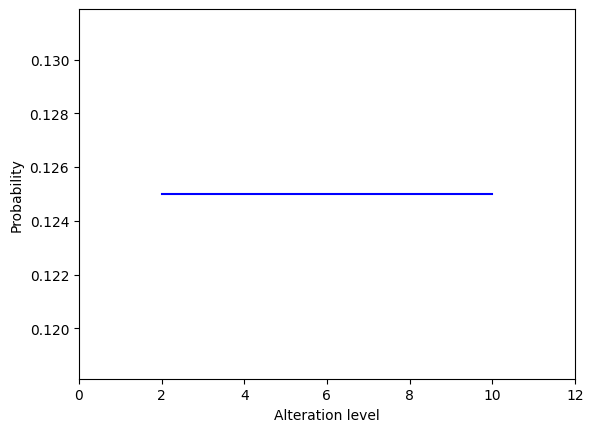
\includegraphics[width=0.9\linewidth]{ImageFiles/ANNRob/unifo_prob}
		\caption{Uniform probability \\ distribution}
		\label{fig:unifo_prob}
	\end{subfigure}%
	\begin{subfigure}{.33\textwidth}
		\centering
		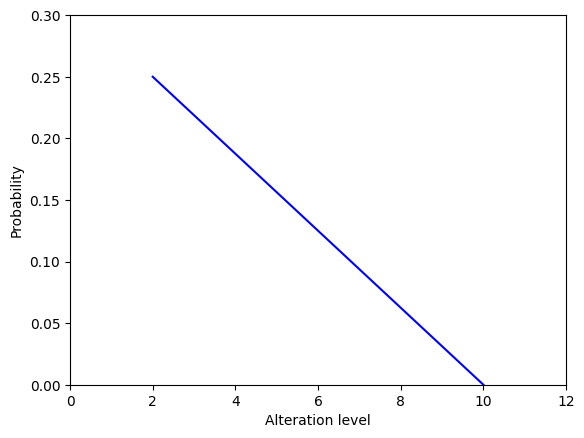
\includegraphics[width=0.9\linewidth]{ImageFiles/ANNRob/lin_prob}
		\caption{Uniform probability \\ distribution}
		\label{fig:lin_prob}
	\end{subfigure}%
	\begin{subfigure}{.33\textwidth}
		\centering
		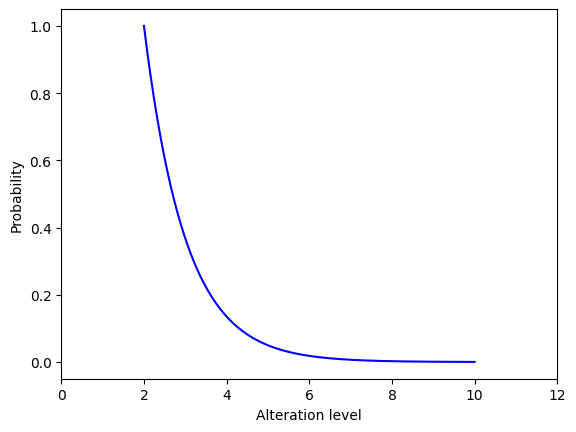
\includegraphics[width=0.9\linewidth]{ImageFiles/ANNRob/exp_prob}
		\caption{Uniform probability \\ distribution}
		\label{fig:exp_prob}
	\end{subfigure}
	\caption{Examples of probability distributions with $L_A=2$ and $U_A=10$}
	\label{fig:prob_examp}
\end{figure}

It is now possible to introduce a third extension of the robustness definition which takes into account the probability distribution of the alteration levels. 

With the consideration of the probability distribution of alteration levels in mind, it is now possible to introduce a third extension of the robustness definition that incorporates this crucial aspect.

\begin{definition}\label{def:rob3} (Robustness extension 3).
	Let $C$ be a classifier, $tol(x)$ a tolerance function and $dep(x)$ a penalization function.
	The robustness $rob_A(C,D) \in [0,1]$ of a classifier $C$ w.r.t. alteration of type A in the range $[L_A, U_A]$ on a dataset $D$ is defined formally as:
	\[
	rob_A(C,D) = \frac{\int_{L_A}^{U_A} [tol(acc(C,D^{A_i}) - \Theta) - dep(acc(C,D^{A_i}) - \Theta)] \cdot p_A(i)\ di}{2} + \frac{1}{2}
	\]
	where $\Theta$ is a threshold referring to minimum accuracy accepted and $p_A$ is probability distribution of the alteration levels.
\end{definition}


\subsection{Fragility}

The approach presented thus far focuses on calculating robustness based on a goodness metric, like accuracy, although it could be any other metric such as precision or recall. The underlying idea is to quantify robustness by measuring the deviation between the metric (e.g., accuracy) and a threshold value $\Theta$. With the latest extension, this metric can also account for how much the accuracy falls below $\Theta$. In essence, this approach measures robustness by quantifying how closely the network is to the ideal scenario.

Alternatively, another way to compute robustness is by performing the inverse calculation, i.e., measuring how far the network deviates from the ideal scenario and using this metric to define the robustness. We call this measure \textit{fragility}. It represents a complementary concept to robustness, both logically and practically. It is possible to define fragility in a similar manner to how we have defined robustness.

\begin{definition} (Fragility).
	Let $C$ be a classifier, $tol(x)$ a tolerance function and $dep(x)$ a penalization function.
	The fragility $fr_A(C,D) \in [0,1]$ of a classifier $C$ w.r.t. alteration of type A in the range $[L_A, U_A]$ on a dataset $D$ is defined formally as:
	\[
		fr_A(C,D) = \frac{\int_{L_A}^{U_A} [dep(acc(C,D^{A_i}) - \Theta) - tol(acc(C,D^{A_i}) - \Theta)] \cdot p_A(i)\ di}{2} + \frac{1}{2}
	\]
	
	where $\Theta$ is a threshold referring to minimum accuracy accepted and $p_A$ is probability distribution of the alteration levels.
\end{definition}

In this definition, the functions $tol$ and $dep$ play the same roles as in \Def~\ref{def:rob3}.$tol$ quantifies the desired level of reward to assign when the accuracy is above the minimum accepted threshold. Conversely, $dep$ refers to the desired penalization when the accuracy falls below $\Theta$. This formula mirrors totally the one used to compute the robustness.

To better understand this metric, an application example will be presented. In particular, both $tol$ and $dep$ will be linear, with $\Theta= 85\%$ and $maxAcc = 100 \%$. The formal expressions for these two functions are as follows:
\[
	tol(acc(C,D^{A_i}) - \Theta) = \begin{cases}
		\frac{min(acc(C,D^{A_i}), maxAcc) - \Theta}{maxAcc - \Theta}  \ for  \ acc(C,D^{A_i}) \ge \Theta\\
		0  \ \ \ \ \ for  \ acc(C,D^{A_i}) < \Theta
	\end{cases}
\]
\[
	dep(acc(C,D^{A_i}) - \Theta) = \begin{cases}
		0 \ \ \ \ \ for \ acc(C,D^{A_i}) \ge \Theta\\
		\frac{\Theta - min(acc(C,D^{A_i}), maxAcc)}{\Theta - maxAcc} \ for  \ acc(C,D^{A_i}) < \Theta
	\end{cases}
\]

\Fig~\ref{fig:frag_example} provides a graphical illustration of the operations involved in the metric. This formula underlines a different aspect, the idea here is to measure a "badness" property of the network.

\begin{figure}[h]
	\centering
	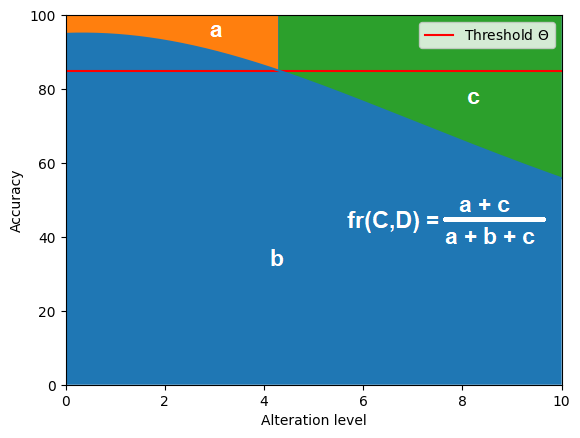
\includegraphics[width=0.7\linewidth]{ImageFiles/ANNRob/frag_example}
	\caption{Example of fragility computation with $\Theta=85\%$ and $maxAcc = 100\%$}
	\label{fig:frag_example}
\end{figure}

Now, robustness can be directly calculated from fragility using the following formula:
\[
	rob_A(C,D) = 1 - fr_A(C,D)
\]

As mentioned earlier, this method is entirely equivalent to computing robustness directly. The choice between the two approaches can be made arbitrarily, depending on the desired aspect to emphasize or measure.